\documentclass[a4paper,12pt]{memoir}
%
%\usepackage{diagbox} %для таблиц
\usepackage{tikz}

\usetikzlibrary{chains, shapes.misc, matrix}
%

\usepackage{listingsutf8} % это лучше, чем verbatim
\usepackage{msiu_term_work}

\lstset{language=Ruby,inputencoding=utf8/koi8-r,basicstyle=\small,
	stringstyle=\ttfamily,xleftmargin=1cm}

\begin{document}
	\renewcommand{\contentsname}{{\Large{Содержание}\hfill}}

	\title{Веб-технологии}
	{Разработка информационной системы библиотеки}
	{141131}
	{А.\+С.~Сазонов}
	{к.т.н., доцент}
	{В.\+Ю.~Радыгин}
	{2017}


	%\setlength{parindent}{0pt}

	\section{Введение}
Данная курсовая работа посвящена разработке интерфейсов информационной системы библиотечных залов,
позволяющий вести учет ее элементов и осуществлять надлежащий контроль связей между ними.
Также будет реализован поиск книг и осуществлена адаптивность для страниц веб-приложения.

Основным инструментом в разработке проекта является фреймворк Ruby on Rails,
написанный на языке программирования Ruby.
Данный фреймворк реализует архитектурный шаблон MVC (Model-View-Controller),
а также обеспечивает поддержку самых востребованных СУБД на сегодняшний день.
В качестве сервера базы данных нами будет использоваться PostgreSQL.

В качестве дополнительных гемов к фреймворку будем использовать гем haml для
более удобной шаблонизации веб-страниц и их отдельных частей. А так же гем
cocoon который поможет нам управлять вложенными формами.

Для подготовки пояснительной записки применялся набор компьютерной верстки \LaTeX.\

\subsection{Постановка задачи}

\begin{enumerate}
\item
Разработайть и добавить в базовое приложение модели необходимые из предметной области.
Описать требуемые ограничения целлостности.
\item
Организовать адаптивные интерфейсы редактирования. А так же настроить систему
авторизации и навигации для данных интерфейсов.
\item
Реализовать поиск книг по всем ее полям, а также всем полям доступных ей объектов.
\end{enumerate}

	%\section{Теоретические аспекты и описание используемых структур данных и применяемых алгоритмов}

Этот раздел содержит рекомендации по оформлению пояснительной записки
и примеры использования различных \LaTeX-конструкций. При подготовке
реального отчёта о выполненной работе данный раздел, естественно, должен
быть опущен.

\subsection*{Общие замечания по структуре курсовой работы}

Обычно в любой работе должно быть \emph{не менее} трёх разделов. Приложение
(или приложения) с текстами программ \emph{не должны} составлять б\'{о}льшую
часть работы. Хорошо, когда в работе имеются таблицы, рисунки или диаграммы,
«снимки экрана» и математические формулы. Возможна, например, такая
структура работы:

\begin{itemize}
\item введение, содержащее постановку решаемой задачи (или задач);
\item изложение необходимых для решения задачи теоретических аспектов;
\item описание используемых структур данных и применяемых алгоритмов;
\item возможные обобщения рассматриваемой задачи;
\item приложения с фрагментами программ;
\item список литературы и интернет-ресурсов.
\end{itemize}

\subsection*{Рекомендации по использованию \LaTeX}

Для подготовки пояснительной записки следует применять \LaTeX\ и пакет
\texttt{memoir}. Настоятельно рекомендуется использовать в исходных
\TeX-файлах кодировку \texttt{UTF-8}. При этом длина большей части строк в
этих файлах не должна превосходить 79 символов. Рекомендуется
использовать только те команды переключения шрифтов, которые поддерживаются
пакетом \verb|memoir| без опции \verb|oldfontcommands|.

При создании pdf-файла используются головной файл \texttt{paper.tex} и
стилевой файл \texttt{msiu\_term\_work.sty}, в котором подключаются
дополнительные
пакеты, определяются размеры полей, стиль оформления страниц и целый ряд иных
параметров и макросов, включая макрос, задающий титульный лист пояснительной
записки. В компьютерных классах МГИУ стилевой файл постоянно обновляется,
поэтому при подготовке пояснительной записки на домашнем компьютере необходимо
использовать последнюю версию этого файла.

При наборе русского текста перед знаками препинания пробел не ставится,
а после них~--- ставится всегда. Следует использовать букву «ё»,
кавычки-ёлочки
(например, \verb|«Информационные технологии и моделирование»|) и
прямой шрифт при наборе единиц измерения (кг, м/сек${}^2$).
При записи инициалов людей рекомендуется применять «сверхтонкий пробел»
(\verb|\+|) между именем и отчеством и «неразрывный пробел» (\verb|~|) между
отчеством и фамилией: \verb|И.\+И.~Иванов|.

Следует использовать по назначению тире
(---), «указатель диапазона» (--), дефис (-) и математический знак «минус»
($-$). Перед тире рекомендуется ставить «неразрывный
пробел», а после него~--- обычный: \verb|после него~--- обычный|. Указатель
диапазона применяется, например, при указании страниц: стр. 15--17
(набирается как \verb|стр. 15--17|). Для набора дефиса необходим минус:
\verb|объектно-ориентированный|, а для получения знака операции  «минус»
требуется применять математический режим: число $-2$ набирается как
\verb|$-2$|.

Сокращения словосочетаний «и так далее» и «и тому подобное», которые
завершают предложение, набираются так: \verb|и~т.\,д.|, \verb|и~т.\,п.|
Не рекомендуется использовать подобные сокращения для словосочетаний,
находящихся в середине предложения. Для набора нумерованных списков
целесообразно использовать окружение \verb|\enumerate| в~следующем виде:
\verb|\begin{enumerate}[1)]|.
Стандартный стиль оформления рисунков и таблиц~--- использование окружений
\verb|figure| и \verb|table|. При этом обязательно следует применять макрос
\verb|caption| для набора подписи.

При наборе математических формул следует нумеровать только те из них, на
которые имеются ссылки. Для получения полужирного шрифта в математических
формулах можно применять команду \verb|\bm|: $\pi \ne \bm\pi$.

О наборе математики мы уже говорили весьма подробно, поэтому сейчас
ограничимся лишь двумя примерами. Следующий код
\begin{small}
\begin{verbatim}
$$\int\limits_a^b\frac12 (1+x)^{-3/2}dx=
\left.-\frac{1}{\sqrt{1+x}}\right|_a^b$$
\end{verbatim}
\end{small}
\noindent позволяет получить формулу

$$\int\limits_a^b\frac12 (1+x)^{-3/2}dx=
\left.-\frac{1}{\sqrt{1+x}}\right|_a^b$$

Приведённый ниже фрагмент кода из книги~\cite{roganov-jurists}
является более сложным.
\begin{small}
\begin{verbatim}
Рассмотрим сначала одну из самых простых функций~$y=x^{2}$. Обычно правую
часть в аналитической записи функции обозначают через $f(x)$. Итак, у нас
$f(x)=x^{2}$. Заметим, что значение этой функции в точке $x_{0} = 2$ равно
$y_{0} = 4$, и возьмём на оси $X$ бесконечную последовательность точек с
координатами $x_{n}=2-1/2^{n - 1}$: $x_{1}=2-1=1$; $x_{2}=2-1/2=3/2$;
$x_{3}=2-1/4=1 3/4$; $\ldots$

\noindent
Эта последовательность, как мы выяснили в \S1, имеет предел, равный двум:
$\displaystyle\lim_{n \to \infty } x_n = 2$. Найдём значения функции
$f(x)$ в выбранных точках:
$$\displaylines{
y_1=f(x_1)=f(1)=1;\cr
y_2=f(x_2)=f\left(\dfrac32\right)= \dfrac94;\cr
y_3=f(x_3)=f\left(\dfrac74\right)=\dfrac{49}{16};\cr
\ldots\ldots\ldots\ldots\ldots\ldots\ldots\ldots\ldots;\cr
y_n=f(x_n)=f\left(2-\dfrac{1}{2^{n-1}}\right)=
\left(2-\dfrac{1}{2^{n-1}}\right)^2=4-\dfrac{1}{2^{n-3}}+\dfrac{1}{2^{2n-2}}.
}$$
\end{verbatim}
\end{small}
\noindent Вот во что он превращается:

Рассмотрим сначала одну из самых простых функций~$y=x^{2}$. Обычно правую
часть в аналитической записи функции обозначают через $f(x)$. Итак, у нас
$f(x)=x^{2}$. Заметим, что значение этой функции в точке $x_{0} = 2$ равно
$y_{0} = 4$, и возьмём на оси $X$ бесконечную последовательность точек с
координатами $x_{n}=2-1/2^{n - 1}$: $x_{1}=2-1=1$; $x_{2}=2-1/2=3/2$;
$x_{3}=2-1/4=1 3/4$; $\ldots$

\noindent
Эта последовательность, как мы выяснили в \S1, имеет предел, равный двум:
$\displaystyle\lim_{n \to \infty } x_n = 2$. Найдём значения функции
$f(x)$ в выбранных точках:
$$\displaylines{
y_1=f(x_1)=f(1)=1;\cr
y_2=f(x_2)=f\left(\dfrac32\right)= \dfrac94;\cr
y_3=f(x_3)=f\left(\dfrac74\right)=\dfrac{49}{16};\cr
\ldots\ldots\ldots\ldots\ldots\ldots\ldots\ldots\ldots;\cr
y_n=f(x_n)=f\left(2-\dfrac{1}{2^{n-1}}\right)=
\left(2-\dfrac{1}{2^{n-1}}\right)^2=4-\dfrac{1}{2^{n-3}}+\dfrac{1}{2^{2n-2}}.
}$$

Теперь рассмотрим пример простой таблицы, которая строится с помощью окружения
\verb|tabular|, и состоит из трёх столбцов. Содержимое каждого столбца может
центрироваться (\verb|c|), либо прижиматься к левому (\verb|l|) или правому
(\verb|r|) краям. Символ~\verb|&| указывает на границу между столбцами, а
символы \verb|\\| --- на конец строки таблицы. Следует понимать, что в таблице
вовсе не обязаны присутствовать горизонтальные и вертикальные линии. Вот как
можно задать грамматику, используя именно такую таблицу:

\medskip
\noindent\hspace{2cm}
\begin{tabular}{rll}
$\alpha \rightarrow$ & $ab\beta$\\
$\beta  \rightarrow$ & $\alpha\mid\gamma$\\
$\gamma \rightarrow$ & $\beta\mid\varepsilon$\\
\end{tabular}
\medskip

\noindent Исходный код для получения этой таблицы имеет следующий вид:

\begin{small}
\begin{verbatim}
\noindent\hspace{2cm}
\begin{tabular}{rll}
$\alpha \rightarrow$ & $ab\beta$\\
$\beta  \rightarrow$ & $\alpha\mid\gamma$\\
$\gamma \rightarrow$ & $\beta\mid\varepsilon$\\
\end{tabular}
\end{verbatim}
\end{small}

Более сложной является таблица~\ref{tabl:crayfish}, позаимствованная из книги
С.\+М.~Львовского~\cite{rlatex}. Заметим, что эта таблица снабжена
подписью (caption) и меткой (label), позволяющей ссылаться на неё.

\begin{table}[ht!]
\caption{Известная шутка М.\+М.~Жванецкого}\label{tabl:crayfish}
\begin{center}
\begin{tabular}{|p{5cm}|p{5cm}|}
\hline
\multicolumn{2}{|c|}{\large\textbf{Я видел раков}}\\
\hline
Вчера: & Сегодня: \\
\hline
Маленькие, но по три рубля, но очень
маленькие, но по три, но очень маленькие.
&
Большие, но по пять рублей, но большие, но
по пять рублей, но очень большие,
но по пять.\\
\hline
\end{tabular}
\end{center}
\end{table}

\noindent
Вот каков исходный код таблицы~\ref{tabl:crayfish}:

\begin{small}
\begin{verbatim}
\begin{table}[ht!]
\caption{Известная шутка М.\+М.~Жванецкого}\label{tabl:crayfish}
\begin{center}
\begin{tabular}{|p{5cm}|p{5cm}|}
\hline
\multicolumn{2}{|c|}{\large\textbf{Я видел раков}}\\
\hline
Вчера: & Сегодня: \\
\hline
Маленькие, но по три рубля, но очень
маленькие, но по три, но очень маленькие.
&
Большие, но по пять рублей, но большие, но
по пять рублей, но очень большие,
но по пять.\\
\hline
\end{tabular}
\end{center}
\end{table}
\end{verbatim}
\end{small}

Наиболее правильным вариантом включение изображения (формата \verb|png| или
\verb|jpg|)
в документ является использование окружения \verb|figure|, что
даёт возможность использовать подписи и нумеровать рисунки.

\begin{figure}[ht!]
\begin{center}
\includegraphics[scale=0.6]{images/msiu_logo}
\end{center}
\vspace*{-8mm}
\caption{Логотип МГИУ}\label{fig:msiu_logo}
\end{figure}

\newpage

Исходный код, использованный для включения логотипа МГИУ,
изображённого на рис.~\ref{fig:msiu_logo}, таков:

\begin{small}
\begin{verbatim}
\begin{figure}[ht!]
\begin{center}
\includegraphics[scale=0.6]{images/msiu_logo}
\end{center}
\vspace*{-8mm}
\caption{Логотип МГИУ}\label{fig:msiu_logo}
\end{figure}
\end{verbatim}
\end{small}

Часто бывает полезно включать в документ «снимки экрана», масштабируя
картинку нужным образом. Примером является рис.~\ref{fig:rating}.

\begin{figure}[ht!]
\begin{center}
\includegraphics[width=0.85\hsize]{images/rating}
\end{center}
\caption{Рейтинг}\label{fig:rating}
\end{figure}

Иногда можно воспользоваться возможностями самого \LaTeX'а,
позволяющего создавать «псевдорисунки». Вот исходный код
рис.~\ref{fig:simple}:

\begin{small}
\begin{verbatim}
\begin{picture}(120,80)
% Границы изображения:
\put(0,0){\line(1,0){120}}
\put(0,80){\line(1,0){120}}
\put(0,0){\line(0,1){80}}
\put(120,0){\line(0,1){80}}
%
% Оси координат:
\put(40,25){\begin{picture}(40,40)%
              \put(20,0){\vector(0,1){40}}
              \put(0,20){\vector(1,0){40}}
              \put(40,22){$x$}
              \put(22,40){$y$}
            \end{picture}}
\end{picture}
\end{verbatim}
\end{small}

\begin{figure}[ht!]
\begin{center}
\begin{picture}(120,80)
% Границы изображения:
\put(0,0){\line(1,0){120}}
\put(0,80){\line(1,0){120}}
\put(0,0){\line(0,1){80}}
\put(120,0){\line(0,1){80}}
%
% Оси координат:
\put(40,25){\begin{picture}(40,40)%
              \put(20,0){\vector(0,1){40}}
              \put(0,20){\vector(1,0){40}}
              \put(40,22){$x$}
              \put(22,40){$y$}
            \end{picture}}
\end{picture}
\end{center}
\caption{Простой псевдорисунок}\label{fig:simple}
\end{figure}

Гораздо более интересным является рис~\ref{fig:cos_acos},
исходный код для которого создан с помощью небольшого скрипта,
написанного на языке Ruby и приведённого в приложении.

\begin{figure}[ht!]
\begin{center}
\input{images/cos_acos.tex}
\end{center}
\caption{Графики функций $y=\cos x$ и $y=\arccos x$}\label{fig:cos_acos}
\end{figure}

Один из простейших способов включения в документ листинга программы~---
использование окружения \verb|verbatim|. При этом полезно немного
уменьшить размер используемого шрифта:

\begin{small}
\begin{verbatim}
y1 = 0
begin
  print "x -> "
  y1,y2 = 1,readline.to_i
  while true
    print "x -> "
    x = readline.to_i
    if x == y2
      y1 += 1
    elsif x > y2
      y1,y2 = 1,x
    end
  end
rescue EOFError
  puts "\nКол-во макс. = #{y1}"
end
\end{verbatim}
\end{small}

Часто исходные тексты программ содержат символы табуляции, которые
правильно интерпретируются текстовыми редакторами, но «приводят в
замешательство» \TeX. Для того чтобы получить правильно отформатированный
листинг программы, следует предварительно заменить в ней все символы табуляции
на пробелы либо вручную, либо с помощью утилиты \verb|expand|.

Более правильным способом включения текста программы является использование
окружения \verb|verbatiminput|. При этом
включаемый текст должен быть размещён в отдельном файле, имя которого и
указывается в качестве параметра окружения. Вот пример:

\begin{small}
\begin{verbatim}
\begin{small}
\verbatiminput{programms/binsearch.rb}
\end{small}
\end{verbatim}
\end{small}

Результат выполнения этих команд имеет следующий вид:

\begin{small}
\verbatiminput{programms/binsearch.rb}
\end{small}

	\newpage

	\section{Секция 1}

\begin{itemize}
  \item \verb|Книга| имеющая название, том/часть, номер ISBN и количество экземпляров;
  \item \verb|Автор| определенный фамилией, именем, отчеством, авторским указателем;
  \item \verb|Зал| содержащий краткое название и полное название помещения;
  \item \verb|Стеллаж| с единственным атрибутом -- индекс стеллажа;
  \item \verb|Расположение| представляет собой связующей звено между \verb|Книгой|
  и \verb|Стеллажом|. Помимо технической информации содержит номера полок;
\end{itemize}

\begin{figure}[ht!]
  \begin{center}
    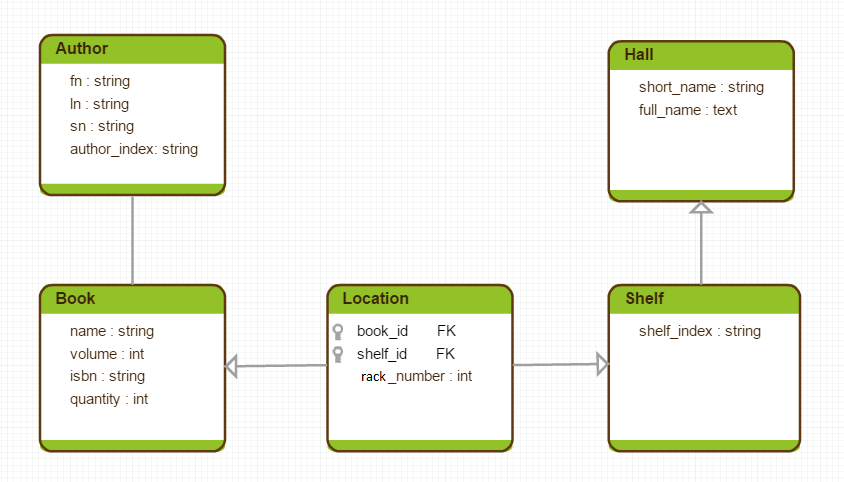
\includegraphics[scale=0.6]{images/erdiagramm.png}
  \end{center}
  \vspace*{-8mm}
  \caption{ER-диаграмма} \label{fig:erdiagramm}
\end{figure}

Вставка кода:
\begin{small}
  \begin{verbatim}
    rails g scaffold Book name:string volume:integer isbn:string quantity:integer
  \end{verbatim}
\end{small}

Вставка исходного кода:
\begin{small}
  \verbatiminput{programms/authors_migrate.rb}
\end{small}

	\newpage

%	\section{Основные интерфейсы}

На предыдущем этапе мы создали вполне работоспособное приложение, но
пользоваться им не удобно и не интуитивно понятно для любого пользователя.
Реализуем интерфейсы редактирования для \verb|Книг| и \verb|Стеллажей|
которые помимо своих собственных сущностей смогут управлять и теми, которые
доступны им по логике применения ИС.

Логически разбобьем всю ИС на две части. Выделим в интерфейс редактирования
стеллажей все что связано с планировкой библиотеки, а также с размещением
книг на стеллажах. Значит нам необходимо работать с сущностями \verb|Зал|,
\verb|Расположение| и непосредственно \verb|Стеллаж|. Во второй интерфейс мы
вынесем оставшиеся сущности связанные с книгами: \verb|Автор|, \verb|Книга|
и \verb|Расположение|.

Для организации интерфейсов мы будем использовать вложенные формы, возможность
использования которых стала доступна при описания нами связей в классах объектов.
Для создания форм связанных моделей используем встроенный метод-хелпер
fields\_for которому передадим форму соответствующей модели созданной
скаффолдом.

Для обеспечения адаптивности, нам необходимо внести в шаблон некоторые
правила каскадных таблиц стилей (CSS), благодаря которым просмотр страницы
будет удобен как на стационарных компьютерах, так и на мобильных устройствах.

Задача адаптивности хоть и совсем непроста, но ее часто необходимо решить.
В условиях подобной необходимости был создан фреймворк Bootstrap.
Это не единственный фреймворк который помогает создать адаптивный
дизайн приложения, но мы будем использовать именно его.

Разобьем наши формы по колонкам используя класс row для контейнера
полей, зададим правила адаптивности колонок и добавим самим полям
класс form-control, тем самым сделаем их более привлекательными.
После этого, в случаем небольшого экрана пользователя, наши формы
будут располагаться в колонку вертикально относительно друг друга.

\begin{small}
\verbatiminput{programms/fields_for.html.haml}
\end{small}

Как можно заметить из примера выше, в шаблоны вложенных форм мы добавим
невидимое поле с идентификатором записи соответствующего объекта. Это
нужно для того, чтобы Ruby on Rails правильно воспринимали получаемые
данные из этих форм: в случае, когда идентификатор не был заполнен,
будет сделана попытка создать новую запись в БД, иначе --- обновить уже
существующую запись в таблице.

Хоть RoR и смогут понять на наличию идентификатора существование сущности
в базе данных, нужно правильно заполнять добавляемые формы на
страницу. Когда создается новый объект поля должны быть изначально
пустыми. А при выборе уже существующего необходимо
заполнять добавленные формы соответствующим им данными.

Поступим следующим образом. Добавив во вложенные формы выпадающий список
с выбором созданных сущностей. При выборе любой из них при помощи JavaScript
мы будем заполнять их данными. Когда же будет выбрано в выпадающем списке
пустое значение (создание новой записи) формы будут очищаться.

Для того, чтобы реализовать задуманное используем технологию AJAX.
AJAX (аббревиатура от «Asynchronous Javascript And Xml») – технология
обращения к серверу без перезагрузки страницы. За счет этого
уменьшается время отклика и веб-приложение по
интерактивности больше напоминает десктоп.

Несмотря на то, что в названии технологии присутствует буква X
(от слова XML), использовать XML вовсе не обязательно.
В мире сложилось так, что часто под AJAX подразумевают также
любое общение с сервером без перезагрузки
страницы, организованное при помощи JavaScript. Хотя в формально
не все такие запросы считаются ajax-запросами.

Создадим отдельный экшен, который будет возвращать ответ клиенту в
формате \texttt{js}, так не будет происходить перезагрузки страницы.

В папке представлений создадим файл с coffee-скриптом имеющий название
соответствующиего ему экшена. Именно этот скрипт
будет исполнен в ответ за запрос
с клиентской части.
Поручим ему очистку и заполнение форм
в зависимости от реакции контроллера.

Осталось добавить ajax-запрос при самом изменении выпадющего списка.
В папке \texttt{javascript} откроем файл общих скриптов для
страниц нашего интерфейса и при помощи библиотеки jQuery
создадим обработчик события изменения выпадющего списка,
который будет отправлять в контроллер выбранное значение
по схеме AJAX. В случае интерфейса книг такой обработчик
может быть написан так:
\begin{small}
\verbatiminput{programms/fill_nested_fields.coffee}
\end{small}
\noindent
Помимо выбранного значения отправляется также уникальный фрагмент имени
самой формы в DOM-структуре страницы по которому конечный скрипт
будет определять точную форму для заполнения данными.

Используем метод гема cocoon для ссылки добавления и удаления
самой вложенной формы на
страничку; использование этого гема сильно
облегчает нашу работу, ведь
с ним нам не нужно самим писать код для создания кнопки добавления форм и
заботиться о том, чтобы rails смогло корректно обработать их,
также не нужно будет организовывать методы удаления связей между объектами.

Для улучшения внешнего вида добавим несколько правил оформления стилей.
В результате форма редактирования книги имеет такой вид:
\begin{figure}[ht!]
\begin{center}
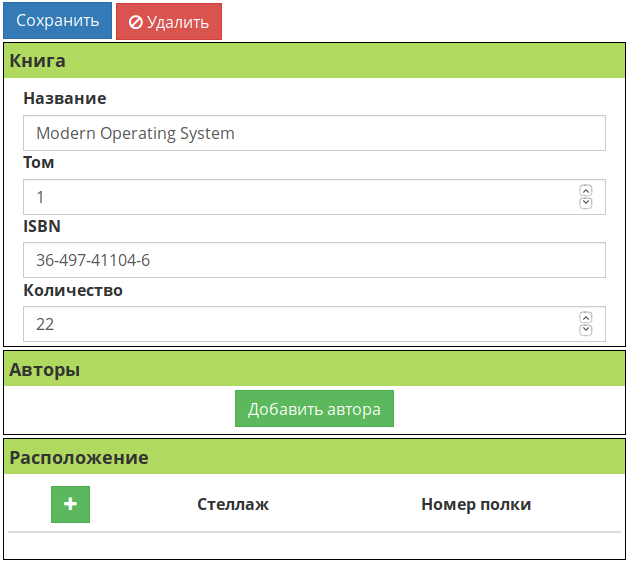
\includegraphics[scale=0.75]{images/book-form2.png}
\end{center}
\vspace*{-8mm}
\caption{Форма редактирования книги} \label{fig:book-form2}
\end{figure}

Закончив с настройкой вложенных форм можно перейти к оформлению списков
книг и стеллажей. Необходимо сделать так, чтобы в описании одной сущности
была вся информация о ней, а так же о сущностях которые ей доступны.

Будем применять относительно новую технологию в CSS именуемой flex-box.
Контейнеры с его свойствами будут менять исходя из размеров экрана.
Подобные технологии получили название Отывчивых (Responsive) и их
главное отличие от Адаптивных (Adaptive) в том, что они не используют
медиа-запросы и не привязываются к конкретным значениям ширины и высоты.
Две эти технологии направлены на решение одной задачи и выбор использования
одной из них - дело вкуса и предпочтений. В руках умелого верстальщика
оба этих инструмента могут использоваться в одном проекте.

Создав подобные списки можно заняться их внешним видом более детально.
Украсим их стандартными css-правилами и корректно переведем все
необходимые строки на русский язык. Добавим навигацию в верхнюю
часть страницы в виде «хлебных крошек» (breadcrumbs) с помощью
которой пользователь без труда будет ориентироваться
в структуре приложения.

Навигационная цепочка
«Хлебных крошек» --- элемент навигации
по веб-сайту, представляющий собой путь по сайту от
его «корня» до текущей страницы, на которой находится пользователь.

Название «Хлебные крошки» является иронической отсылкой к
немецкой сказке «Гензель и Гретель», в которой дети,
когда их завели в лес во второй раз, не смогли найти
обратную дорогу, так как на этот раз вместо маленьких камешков они
оставляли за собой хлебные крошки, впоследствии склёванные лесными птицами.

Существует огромное множество реализаций подобных систем навигации.
Их число определяется тем, что вместе с прикладной значимостью
«хлебные крошки» --- элемент дизайна сайта, который может подстраиваться
под окружения любого приложения. В нашем случае мы построим
такую цепочку просто разделив ее элементы символом-стрелочкой.

%\newpage
Конечный результат для списка \verb|Стеллажей| можно видеть на
следующем изображении:

\begin{figure}[ht!]
\begin{center}
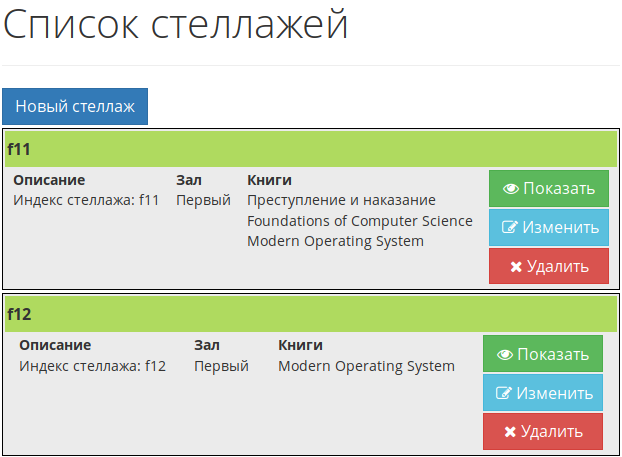
\includegraphics[scale=0.75]{images/shelves-index.png}
\end{center}
\vspace*{-8mm}
\caption{Список стеллажей} \label{fig:shelves-index}
\end{figure}

Разделение ответственностей и обязанностей между ролями тоже
входит в задачи нашей информационной системы. Допустим, что
необходимо допустить всего две основные роли: администратор и оператор.

Обозначим доступные им возможности ИС. В случае администратора все
банально и просто - он может все (подобную роль необходимо назначать
пользователям с осторожностью, ведь у них будет полный доступ к приложению!).
Оператору мы позволим использовать возможности интерфейсов редактирования
\verb|Книг| и \verb|Стеллажей| в полной мере, но полностью запретим
ему доступ к части администрирования. Незарегистрированному пользователю
позволим просматривать списки стеллажей и книг.

В Rails подобные ограничения необходимо выполнить в виде
методов-фильтров, которые будут запускаться перед или после
определенными экшенами
контроллера. Разместить их необходимо разумеется в них.

\newpage

Чтобы не загромождать модели определениями каждой из необходимых нам
функций, мы будем использовать возможности объекта Proc (создадим его потомка
lambda для лямбда-функций) определяя права текущего пользователя. Контроллер
для \verb|Книг| преобразуется следующим образом:

\begin{small}
\verbatiminput{programms/book_controller.rb}
\end{small}

Добавленная лямбда-функция в классе контроллера находится на третей строчке
и ее начало обозначается стрелочкой. На предыдущих строках
описан фильтр позволяющий просматривать списки книг и описание отдельных
экземпляров. Сам этот метод реализован в базовой версии проекта
и поэтому рассматриваться нами не будет.

На данном этапе приложение включает в себя адаптивно реализованные
интерфейсы для \verb|Книг| и \verb|Стеллажей| с вложенными
формами. Настроена система навигации
и авторизации. Проект полностью русифицирован.

%	\newpage
%
%	\section{Поиск книг}

Хоть и список книг
организован достаточно компактно, при большом количестве книг нахождение
конкретного экземпляра в нем будет довольно проблематично.
Поэтому следующее что мы сделаем --- реализуем поиск по книгам.

Система поиска должна получать и правильно обрабатывать все атрибуты
объекта \verb|Книга|, а также все те атрибуты моделей к которым
можно добраться по транзитивным связям. \verb|Книге| доступен
\verb|Автор|, \verb|Стеллаж|, модель \verb|Расположения| книг на
стеллажах и \verb|Зал| в котором должен находится стеллаж.
Тем самым поиск книг будет затрагивать поля всех существующих на
данный момент моделей в нашем приложении.

На первый взгляд это может показаться чрезмерным, но на деле это довольно удобно.
Благодаря такой обширности настроек поиска, в случае надобности, можно
получить книги содержащиеся в конкретном зале или те книги, которые стоят
на одной полке конкретного стеллажа.

Снача построим представление будущего поиска. Создание форм
поручим встроенному хелперу \texttt{form\_tag.}
Перенесем формы из созданными нами ранее интерфейсов.
Для того чтобы Rails
правильно подобрал данные из форм поиска то изменим название
каждой из них в соотвутствии с данным шаблоном:
\begin{small}
\begin{verbatim}
  <тип данных>_field_tag 'search[<сущность>][<атрибут>]', nil
\end{verbatim}
\end{small}
\noindent
так параметры в контроллер придут в структурированном виде, который
облегчит написание самого метода поиска.

Создадим в контроллере книг новый экшен поиска (и пропишем в
файле \texttt{route.rb} новый маршрут к нем по протоколу get).
Новый экшен будет проверять параметры на содержание ключа 'search'
и, в случае его обнаружения, запускать метод поиска расположенного в
модели книг и выводить его результат на страницу.

Чтобы передать методу поиска только те параметры которые могут придти
в качестве запроса (параметры могут быть вручную изменены злоумышленниками
желающих понизить производительность вычислений) то используем
механизм фильтра параметров называющийся \texttt{strong parameters}.
Создадим такой фильтр:
\begin{small}
\verbatiminput{programms/search_params.rb}
\end{small}

Займемся реализацией самого поиска. Как было указано выше, мы поместим
его в модель \verb|Книги| согластно MVC-структуре приложения.
На вход он будет принимать отфильтрованные контроллером параментры.
Благодаря тому, как мы организовали представление, они всегда будут
структурированны в хеше, где ключем является имя сущности, а значением
выступает вложенный хеш с ее атрибутами.

Значит все что нам нужно это изначально составить запрос
на все книги и, по мере
наличия значения определенного атрибута, добавлять к этому запросу
соответствующие ограничения. Мы работаем с вложенными атрибутами,
значит при инициализации первичного запроса нам необходимо подгрузить еще
таблицы связанных сущностей. Так мы обеспечим себе возможность
поиска не только по полям \verb|Книги|, но и по связанным с ней объектам.

\begin{small}
\verbatiminput{programms/search.rb}
\end{small}

Теперь можно позаботится о том, как мы будем отображать результаты
выполненного поиска. Хорошим вариантом будет использование таблицы
ведь в ней можно компактно уместить всю информацию о книгах.

Заголовками столбцом будут названия атрибутов, а в отдельных ячейках
запишем соответствующие заголовкам данные найденных книг. Поместим
описание каждой книги на отдельную строку таблицы. Для
того, чтобы она стала более привлекательной дадим ей определенный
фреймворком Bootstrap класс \texttt{table}, а
также класс \texttt{table-striped}. При помощи последнего строки таблицы будут
немного отличаться друг от друга фоновым цветом, что сделает таблицу более
читабельной.

Не станем забывать, что пользователи приложения возможно не будут
иметь большого экрана. В их случае представление информации в таком виде
будет неудобно.

Сделаем таблицу адаптивной. Для этого при создании каждой ячейки мы
запишем соответствующее им название заголовка столба в дата-атрибут.
Само по себе наличие этого атрибута никак не отразится на внешнем виде
табилцы. Поэтому в правилах оформления укажем нашей таблице, что при
достижении ширины экрана пользователя определенной величины мы поместим
содержимое дата-атрибута каждой ячейки перед ней при помощи псевдо-класса
\texttt{:before}, а сами ячейки и строки таблицы
заставим отображаться блоками. Отображение заголовка таблицы мы уберем вовсе:
\begin{small}
\verbatiminput{programms/adaptive-table.sass}
\end{small}

Добавим обтекание контекта из дата-атрибутов и выровнем текст
по правой стороне. Создадим границы у строк таблицы и добавим
отступы сверху и снизу, чтобы отличить данные конкретных
экземпляров книг.

\newpage

Результат поиска будет выглядеть так. Слева показан результат поиска для пользователей с большим экраном,
а справа~--- для тех, чьи устройства не обладают достаточно большим экраном:
\begin{figure}[h]
\begin{minipage}[h]{0.49\linewidth}
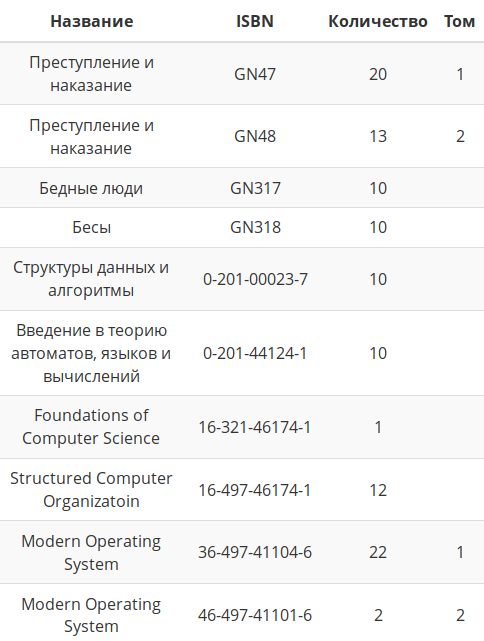
\includegraphics[scale=0.60]{images/search-result2.png} \\ а) Большой экран
\end{minipage}
\hfill
\begin{minipage}[h]{0.49\linewidth}
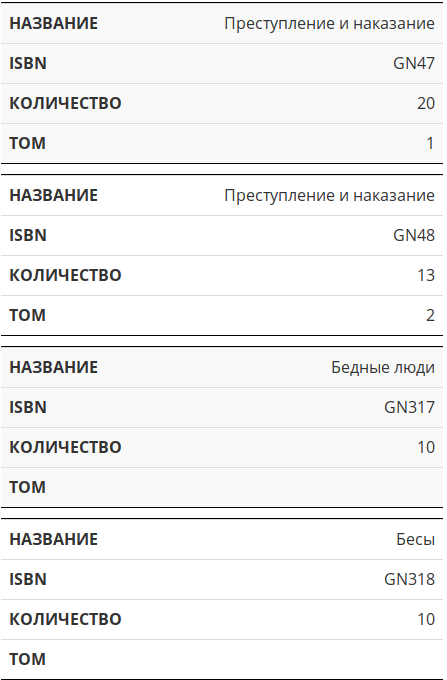
\includegraphics[scale=0.60]{images/search-result-adaptive.png} \\ б) Маленький экран
\end{minipage}
\caption{Адаптивная таблица результатов поиска.}
\label{ris:adaptive-table}
\end{figure}

Теперь немного изменим внешний вид всего приложения. Перенесем боковую
панель на правую сторону и перекрасим заголовки в зеленые цвета.

Откроем файл \texttt{theme.sass} где описана цветовая схема страниц.
В переменной \texttt{navbar-inverse-bg} находится основной цвет залоговков.
В базовой версии проекта уже настроена цветовая зависимость компонентов
страницы от этого цвета. Нам всего лишь необходимо его поменять на желаемый.

Перейдем к описанию стилей для боковой панели. Оно находится в
файле \texttt{sidebar.sass}.

Изначально боковое меню занимает позицию слева от
основного содержимого страницы. Необходимо изменить значения
\texttt{left} на \texttt{right}. Но это еще не все.
При скрытии или при разворачивании меню контейнер для основного содержимого
получал или убирал внутренние поля с левой стороны
в размере ширины бокового меню.

Заменим это поведение на противоположное. Внутренние поля теперь
будут изменяться с правой стороны контейнера.

Само меню переключалось по нажатию небольшой кнопки расположенной
в области основного контента, которая добавляла или удаляла
класс \texttt{toggled} у всей страницы. Тоже перенесем ее
в правую часть родительского контейнера.

Осталось только внести соответствующие изменения в медиа-запрос,
в котором боковое меню при получении страницы класса-переключателя
должно вести себя с точностью до наоборот.

\begin{figure}[ht!]
\begin{center}
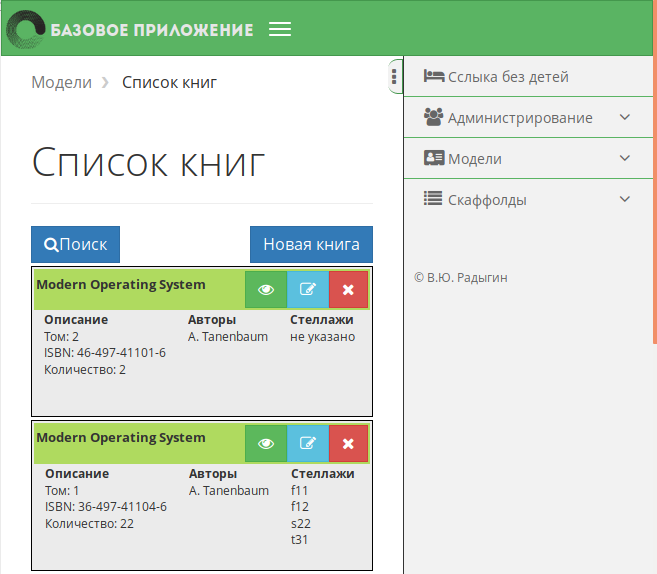
\includegraphics[scale=0.75]{images/sidebar.png}
\end{center}
\vspace*{-8mm}
\caption{Боковое меню справа} \label{fig:sidebar}
\end{figure}

На данном этапе в проекте реализован работоспособный поиск
\verb|Книг|, включая не только ее собственные атрибуты, но и те, которые
доступны ей по транзитивным связям. Результат поиска
оформлен в виде адаптивной таблицы. Выполнено задание по внешнему оформлению
проекта.

%	\newpage

	\section{Заключение}

Поставленная задача решена полностью в соответствии
с поставленными требованиями. В результате получена
полноценная ИС, позволяющая вести учет элементов библиотеки.

Реализованы основные интерфейсы, при помощи которых можно просто и
эффективно управлять содержимым приложения и добавлена функция
поиска книг.

Элементы интерфейсов адаптивны к просмотру на экранах
любого размера.

Разделены обязанности у ролей и выполнено задание по
внешнему оформлению проекта.

В рамках разработки ИС созданы концептуальная и даталогическая
модели предметной области.

	\newpage

	\begin{thebibliography}{}

\bibitem{ruby}
Флэнаган Д., Мацумото Ю.
{\em Язык программирования Ruby.}~---
СПб.: Питер, 2011.

\bibitem{snitko}
Снитко Р.
{\em Мир Rails. Правильное обучение разработке веб-приложений на Ruby On Rails.}~---
2013.

\bibitem{rorapi}
\link{http://api.rubyonrails.org/}~---
Official API of the framework, 11.07.2017

\bibitem{ruby-guides}
\link{http://guides.rubyonrails.org/}~---
Руководства по отдельным составляющим фреймворка Ruby on Rails., 26.07.2017


\bibitem{bootstrap}
\link{http://getbootstrap.com/}~---
Официальная страница фреймворка Bootstrap с описанием
спецификации и руководставами., 26.07.2017


\bibitem{rusrails}
\link{http://rusrails.ru/}~---
Ruby on Rails руководства, учебники, статьи на русском языке., 12.07.2017

\bibitem{kormen}
Т. Кормен.
{\em Алгоритмы: построение и анализ, 2-е изд.}~---
Пер. с англ. --- М., Издательский дом «Вильямс», 2005.

\bibitem{latex}
С.М. Львовский.
{\em Набор и вёрстка в системе \LaTeX, 3-е изд., испр. и доп.}~---
М., МЦНМО, 2003. Доступны исходные тексты этой книги.

\end{thebibliography}

	\newpage

	%\subsection{subsection}
\subsubsection{subsubsection}
\paragraph{paragraph}

Реалицазия структуры \texttt{Queue} и некоторых методов для работы с ней:
\begin{verbatim}
//определение элемента Queue (Queue_Element):
typedef struct Queue_Element{
  int data;
  struct Queue_Element *next;
} Queue_Element;

//определение Queue:
typedef struct Queue{
  struct Queue_Element *head;
  struct Queue_Element *tail;
  int size;
} Queue;

//инициализация Queue:
Queue* Queue_init() {
  Queue *tmp = (Queue*) malloc(sizeof(Queue));
  tmp -> size = 0;
  tmp -> head = tmp -> tail = NULL;
  return tmp;
}

//дабавление элемента:
void Queue_push(Queue *q, int d) {
  Queue_Element *new_element = (Queue_Element*)
                            malloc(sizeof(Queue_Element));
  new_element -> data = d;
  if (q -> head == NULL){
    q -> head = q -> tail = new_element;
    q -> head -> next = q->tail->next= NULL;
  }else{
    q -> tail -> next = new_element;
    q -> tail = new_element;
  }
  q -> size++;
}

//удалаение Queue:
void Queue_free(Queue *q){
  Queue_Element* tmp; int i;
  for (i=0; i < q->size; i++){
    tmp = q -> head;
    (q -> head) = (q -> head -> next);
    free(tmp);
  }
  free(q);
}
\end{verbatim}


\end{document}
